\section{The case $[2 \times 3, 4]_5$}
In the following part a theorem of Eberhards type will be proven for $5$-valent polyhedra. The proof utilizes the already established Eberhards \autoref{thm:eberhard:4} for construction of the new solid.
\begin{theorem}
  Let $p = (p_3, p_4, p_5, \dots, p_n)$ be a given sequence satisfying \autoref{eq_valence_5}, then there exists $r \in \nats$ for which $p + r [2 \times 3, 4]_5$ is $5$-realizable.
  \begin{proof}
    Beginning with equation \autoref{eq_valence_5} one retrieves the following:
    \begin{align*}
      &\sum_{k=3}^n \left( \frac{10}{3} - k \right) p_k = \frac{20}{3} \\
      \implies & \frac{p_3}{3} = \frac{20}{3} + \sum_{k=4}^n \left(k - \frac{10}{3} \right) p_k \geq \frac{20}{3} + \frac{2}{3} \sum_{k=4}^n p_k \\
      \implies & p_3 = \frac{20}{3} + \frac{2}{3} \sum_{k=3}^n p_k \geq - \frac{4}{3} + \frac{2}{3} \sum_{k=3}^n p_k
    \end{align*}
    Therefore one can assume, that $p'_3 := p_3 + \frac{4}{3} - \frac{2}{3} \sum_{k=3}^n p_k \geq 0$ and for $p'_k = p_k$, $(k\geq 4)$ the resulting sequence fullfills:
   \begin{align*}
     \sum_{k=3}^n (4 - k) p'_k =&~ p_3 + \frac{4}{3} - \frac{2}{3} \sum_{k=3}^n p_k + \sum_{k=4}^n (4 - k) p_k \\
     = \frac{4}{3} + \frac{1}{3} p_3 + \sum_{k=4}^n \left(k - \frac{10}{3} \right) p_k =&~ \frac{4}{3} + \sum_{k=3}^n \left(k - \frac{10}{3} \right) p_k = \frac{4}{3} + \frac{20}{3} = 8.
   \end{align*}
   Hence the sequence $p'$ is $4$-realizable by Eberhards Theorem \autoref{thm:eberhard:4}. Let $P'$ be this realization with $e'$ edges and $v'$ vertices. One can now use $P'$ to create a realization with valence $5$ by inserting further triangles and quadrangles. This is done by replacing each edge of the realization by two triangles and each vertex by one square as shown in:

   %TODO.
   \begin{figure}[hptt]\centering
   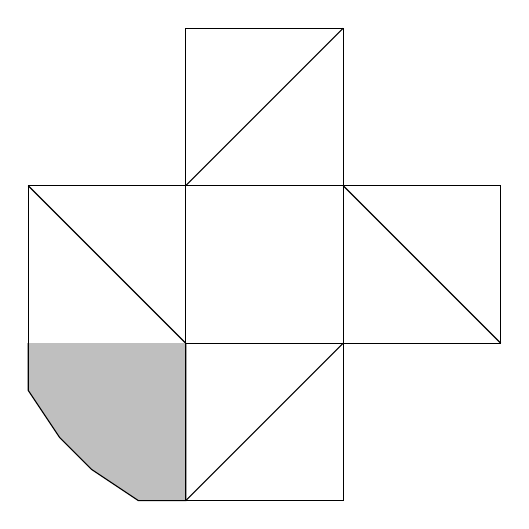
\begin{tikzpicture}[scale=2]
     \draw (0, 1) -- (1, 1) -- (1, 0) -- (2, 0) -- (2, 1) -- (3, 1) -- (3, 2) -- (2, 2) -- (2, 3) -- (1, 3) -- (1, 2) -- (0, 2) -- (0, 1);     
     \draw (1, 1) -- (0, 2);
     \draw (2, 1) -- (1, 0);
     \draw (1, 2) -- (2, 3);
     \draw (2, 2) -- (3, 1);
     \draw (1, 1) -- (2, 1) -- (2, 2) -- (1, 2) -- (1, 1);

     \filldraw[fill=gray!50!white] (0, 1) -- (0, 0.7) -- (0.2, 0.4) -- (0.4, 0.2) -- (0.7, 0) -- (1, 0) -- (1, 1);
   \end{tikzpicture}
   \end{figure}
   The resulting polyhedron $P$ is $5$-valent, let $p''$ be its $p$-vector. It differs from $p$ only by the number of triangles and quadrangles. Since equation \autoref{eq_valence_5} holds for $p$ as well as for $p''$ this means
   \begin{align*}
     & \sum_{k=3}^n \left( \frac{10}{3} - k \right) p_k'' - \sum_{k=3}^n \left( \frac{10}{3} - k \right) p_k = 0 \\
     \implies& \frac{1}{3} (p''_3 - p_3) = \frac{2}{3} (p''_4 - p_4),
   \end{align*}
   hence $p + r [2 \times 3, 4]_5 = p''$ is realizable for some $r \in \nats$.
  \end{proof}
\end{theorem}

